\documentclass[a4paper,twoside,master.tex]{subfiles}
\begin{document}
\lecture{22}{Wednesday, March 04, 2020}{Phase Transitions}

\section{Phase Transitions}
\label{sec:phase_transitions}

Instead of writing down the entropy from first principles, we made a guess as to how non-ideal gasses might behave to modify the free energy. We found that below a ``critical'' temperature, the free energy was not necessarily convex, making the pressure-volume curve no longer monotonic. We found a way to cut this non-monotonic part into sections of equal area, and it turns out that moving along this line corresponds to moving along the convex envelope of the free energy. In the Gibbs free energy, this critical region corresponds to a ``bow-tie'' like the one we saw in a homework problem, and the Maxwell construction cuts the tie. Now we want to know why the convex envelope is correct in the first place.


Recall in if we are in free energy variables and we pick $ T $, $ V $, and $ N $, we can find the corresponding free energy. If the volume is in the critical region, there is a way to further minimize the energy by splitting into two volumes, one in each dip. Once you do that, the total free energy lies on the convex envelope line. The system found an opportunity to lower its free energy by phase separating.


For any volume in that critical range $ V \in [V_1, V_2] $, the system can lower its free energy by splitting into a fraction $\alpha$ at the state point $ V_2 $ and a fraction $ 1 - \alpha $ at $ V_1 $. If it does so, the free energy after splitting is
\begin{equation}
    F_{\text{split}} = \alpha F(V_2) + (1 - \alpha) F(V_1)
\end{equation}
We must also conserve the original volume, so $ V = \alpha V_2 + (1 - \alpha) V_1 $. We can solve this for alpha:
\begin{equation}
    \alpha = \frac{V - V_1}{V_2 - V_1}
\end{equation}
Therefore,
\begin{equation}
    F_{\text{split}} = \frac{V - V_1}{V_2 - V_1} F(V_2) + \frac{V_2 - V}{V_2 - V_1} F(V_1)
\end{equation}
At the endpoints, one of the terms vanishes, and between the end points, this is a linear combination of the endpoint values. Therefore, this phase separation energy is the line connecting the critical points. This is how phase transitions happen. In the critical region, weird things happen. The compressibility becomes negative, and this is a violation of the stability criteria we established a few lectures ago. This is what allows the system to no longer stay homogeneous.


This construction now allows us to construct phase diagrams (\Cref{fig:lec_22_phase_diagram}):

\begin{figure}[h]
    \centering
    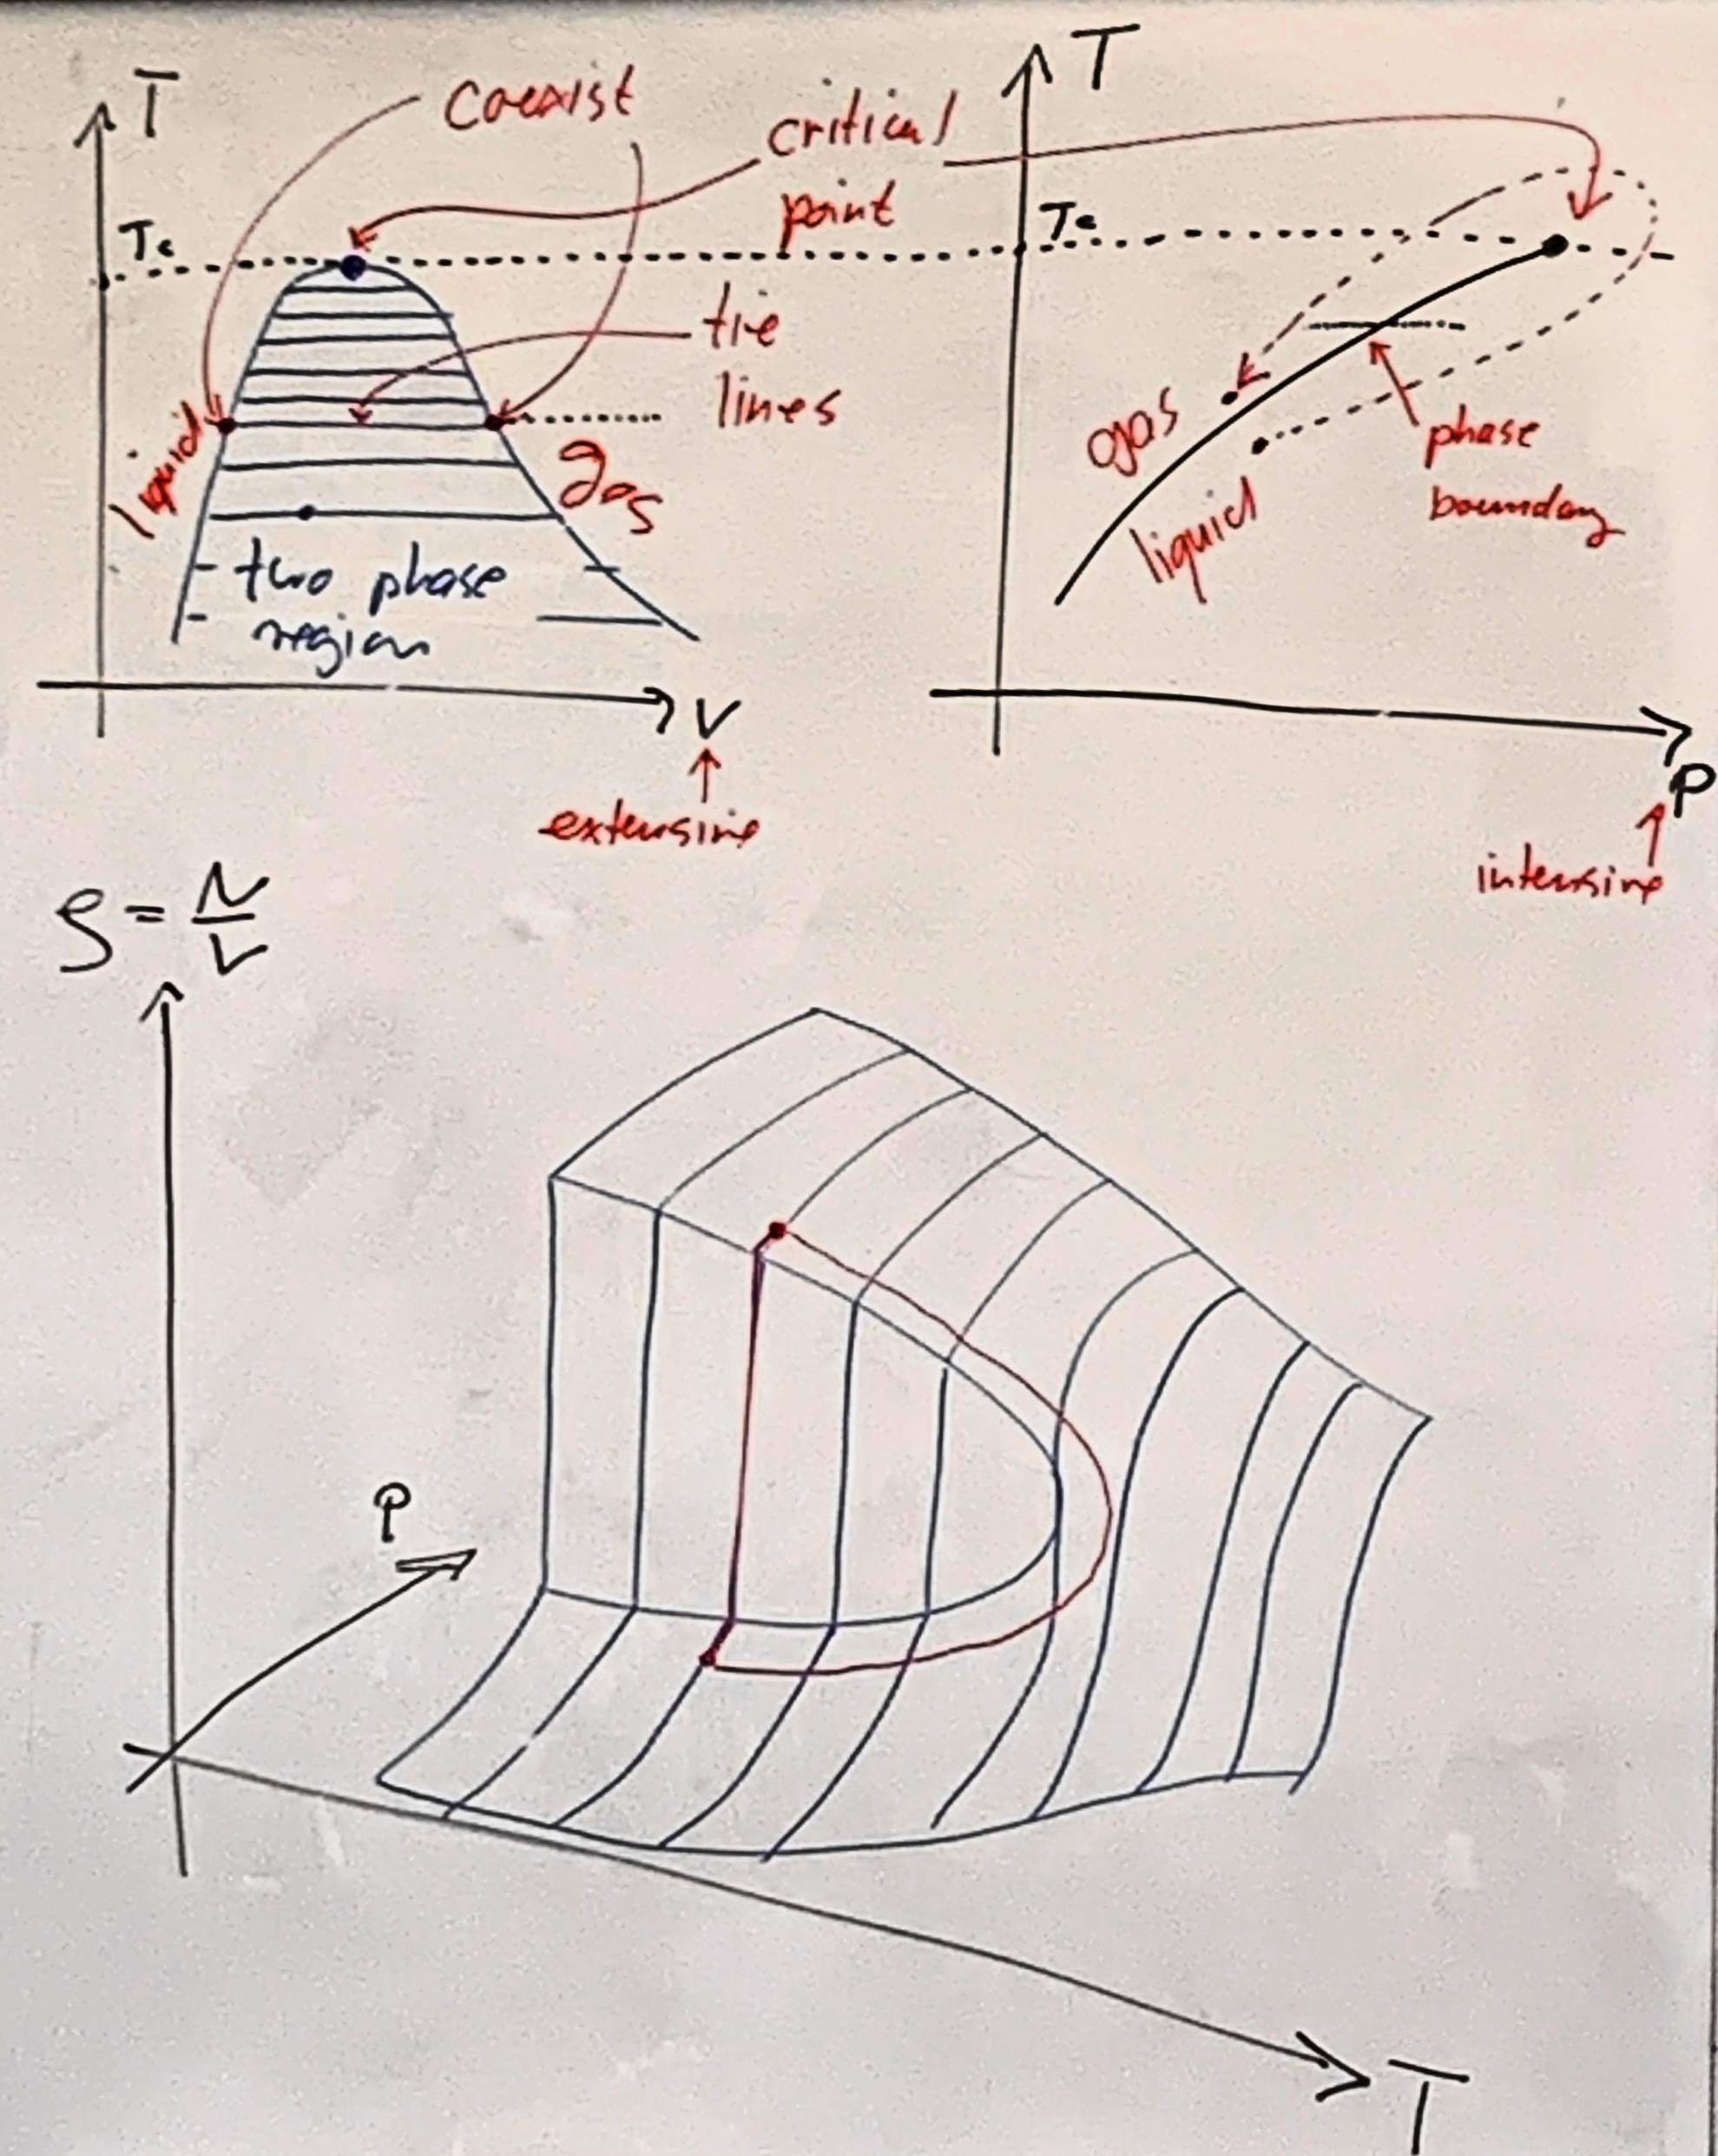
\includegraphics[width=\textwidth]{figures/lec_22_phase_diagram.png}
    \caption{A typical phase diagram}
    \label{fig:lec_22_phase_diagram}
\end{figure}

\subsection{Latent Heat}
\label{sub:latent_heat}

There is a finite amount of heat which goes into or comes out of the system when it experiences a 1st order phase transition:
\begin{equation}
    \Delta Q = T \Delta S
\end{equation}
Considering constant $ T $ and $ N $,
\begin{equation}
    \dd{S} = \eval{\pdv{S}{V}}_{T,N} \dd{V} = \eval{\pdv{P}{T}}_{V,N} \dd{V}
\end{equation}
Therefore
\begin{equation}
    \Delta S = \int_{V_1}^{V_2} \dd{V} \eval{\pdv{S}{V}}_{T,N} = \int_{V_1}^{V_2} \dd{V} \eval{\pdv{P}{T}}_{V,N} = \eval{\pdv{P}{T}}_{V,N} \int_{V_1}^{V_2} \dd{V} = \eval{\pdv{P}{T}}_{V,N} \Delta V
\end{equation}
We can therefore write
\begin{equation}\label{eq:clausius_clapeyron_equation}
    \frac{\Delta S}{\Delta V} = \eval{\pdv{P}{T}}_{\text{phase boundary}}\tag{Clausius Clapeyron Equation}
\end{equation}

\begin{ex}
    Let's look at an example using the phase diagram of water (see \Cref{fig:lec_22_water_phase}). On the phase boundary between gas and liquid, the slope is positive, so $ \frac{\Delta S}{\Delta V} > 0 $. This implies that evaporation increases the entropy. However, if we look at the liquid-ice boundary, the slope is negative, which tells us that freezing water lowers the entropy (ice is an ordered crystal). This also implies that when ice freezes, it expands.

\end{ex}
\begin{figure}[h]
    \centering
    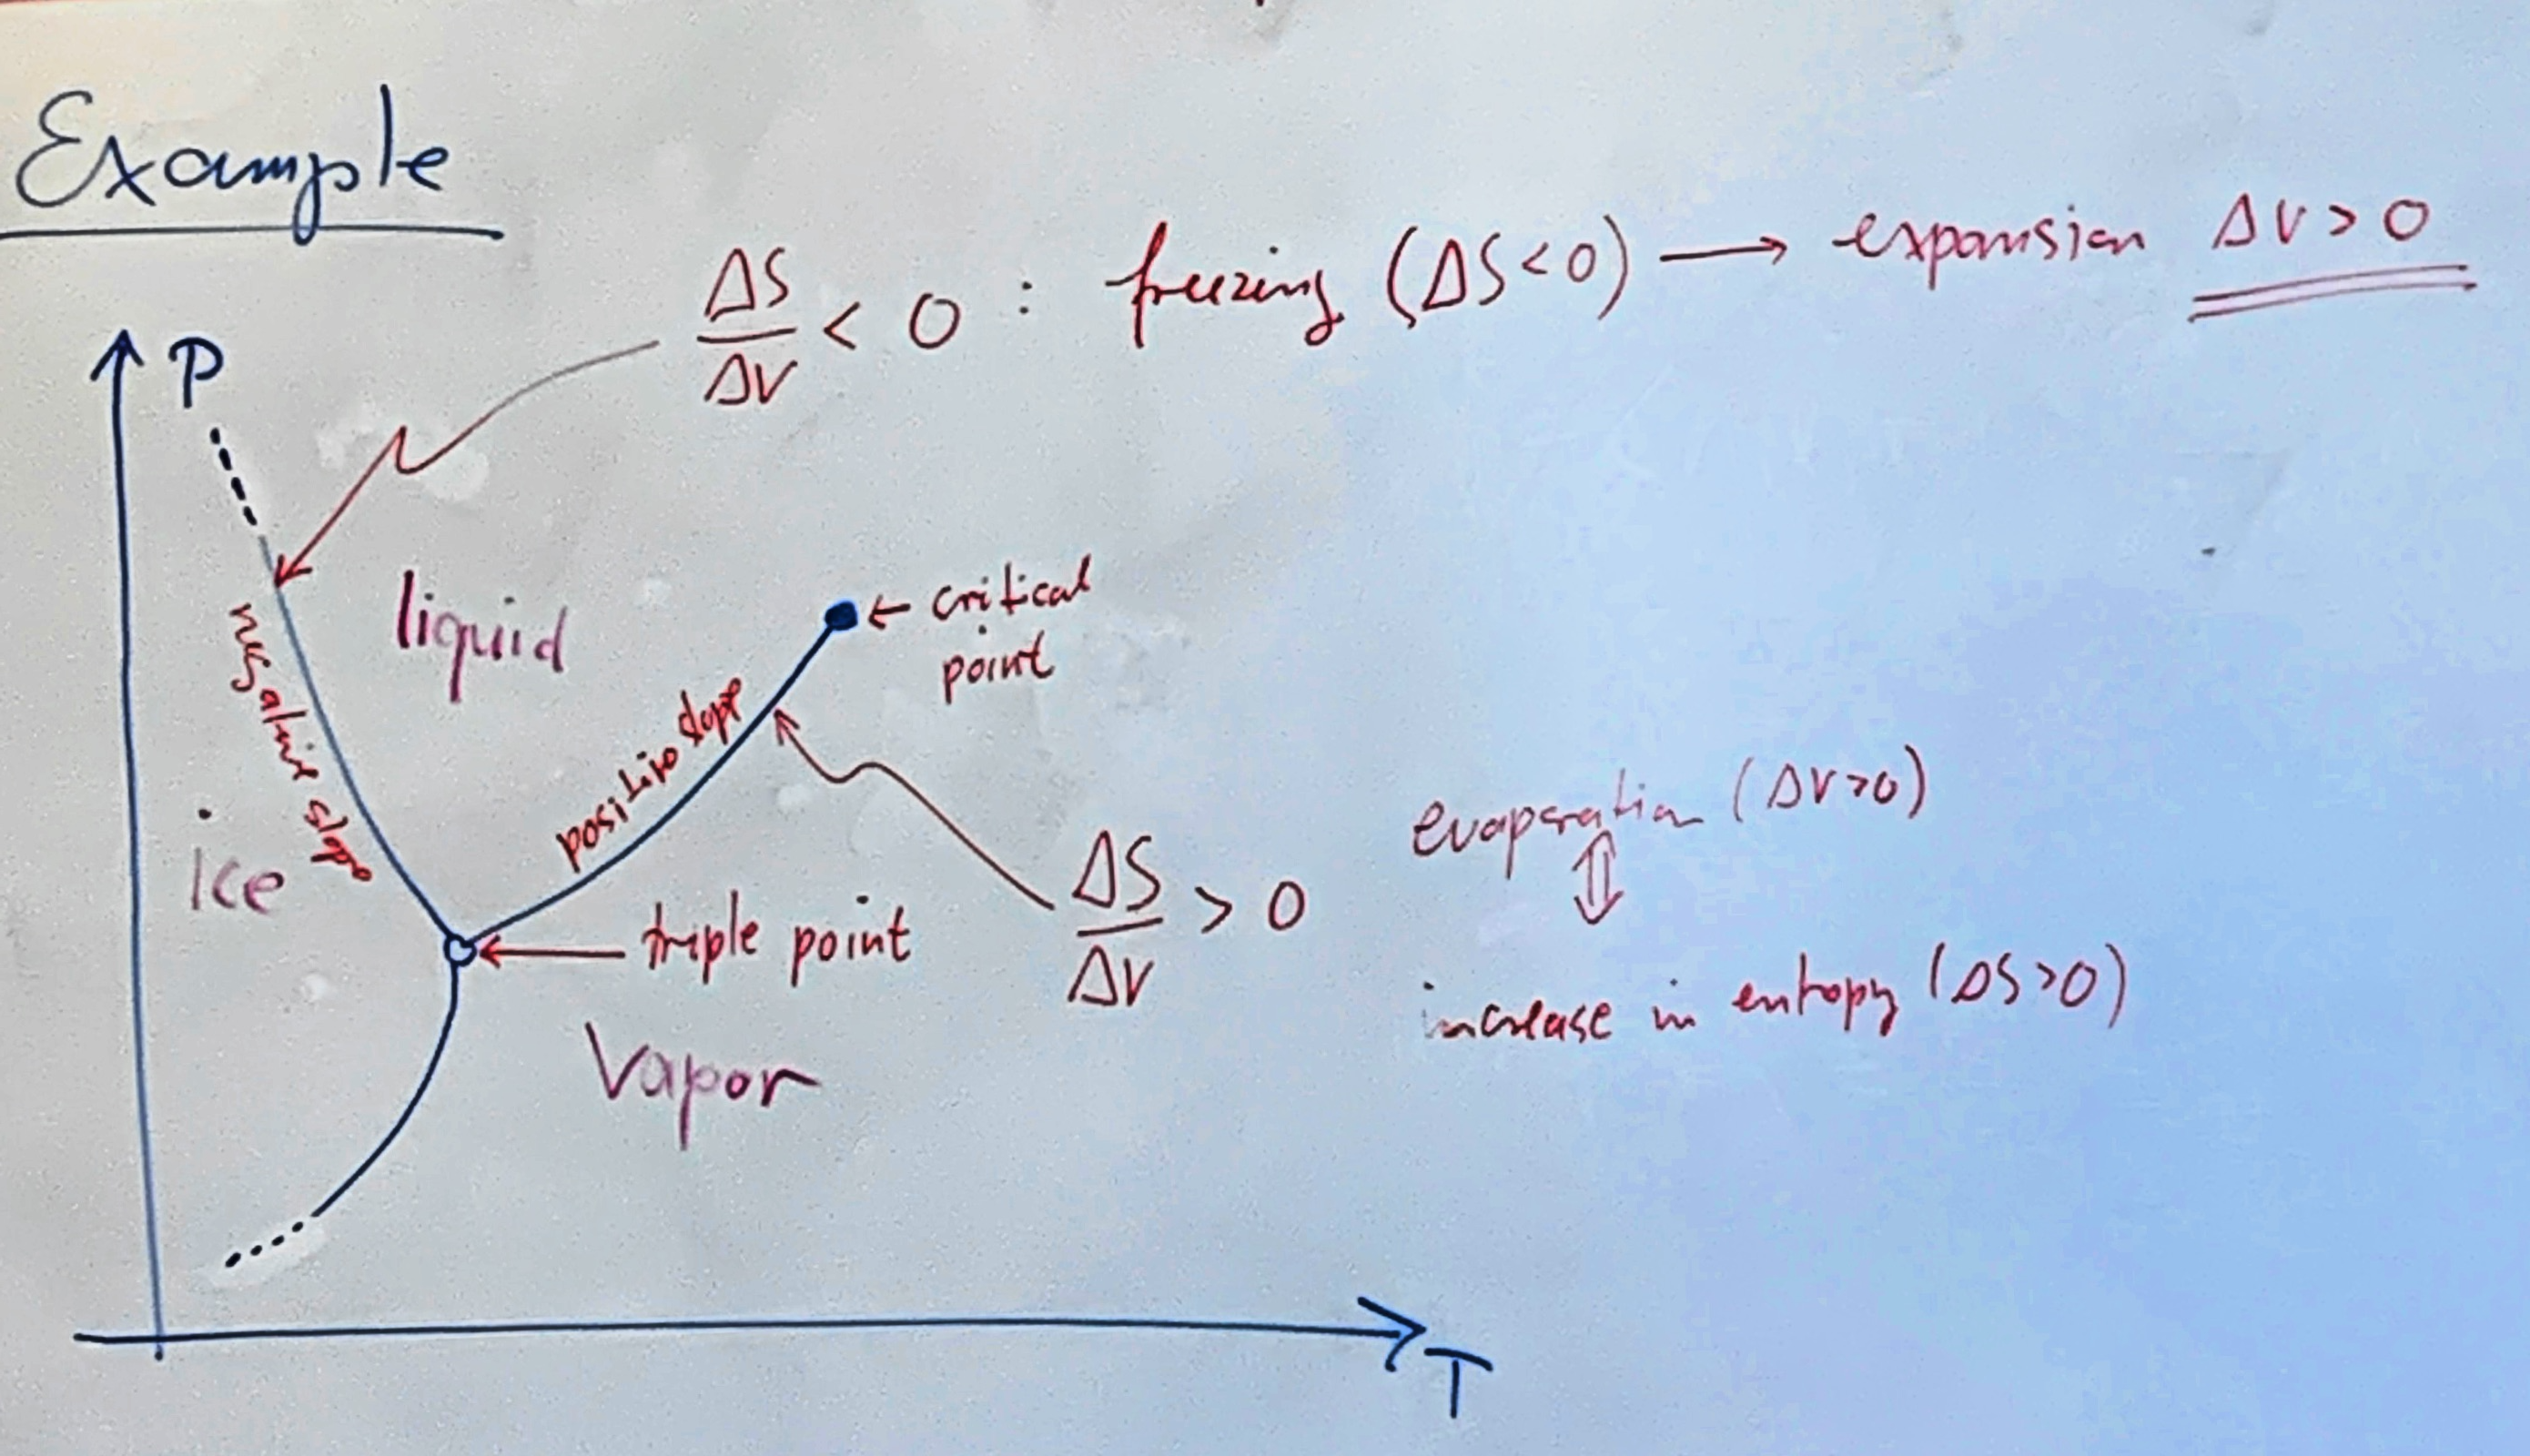
\includegraphics[width=\textwidth]{figures/lec_22_water_phase}
    \caption{Phase Diagram of Water}
    \label{fig:lec_22_water_phase}
\end{figure}

\end{document}
